
\begin{flushleft}

\begin{itemize}
	\item Port forwarding is a form of \textbf{NAT} (Network Address Translation). 
	\item With port forwarding, traffic of a server is forwarded to a different port on the same machine, or to a port on a different machine. 
	\item This is used \textbf{“hide”} a server behind another machine, or to provide access to a service on an alternate port.
	\item Eg: 
	\begin{itemize}
		\item Ssh server with IP address "192.168.0.108" can configure rich rule such that traffic coming from client address "192.168.0.106" at port 2020 is forwarded to port 22 on ssh server.
	\end{itemize}
	\begin{figure}[h!]
		\centering
		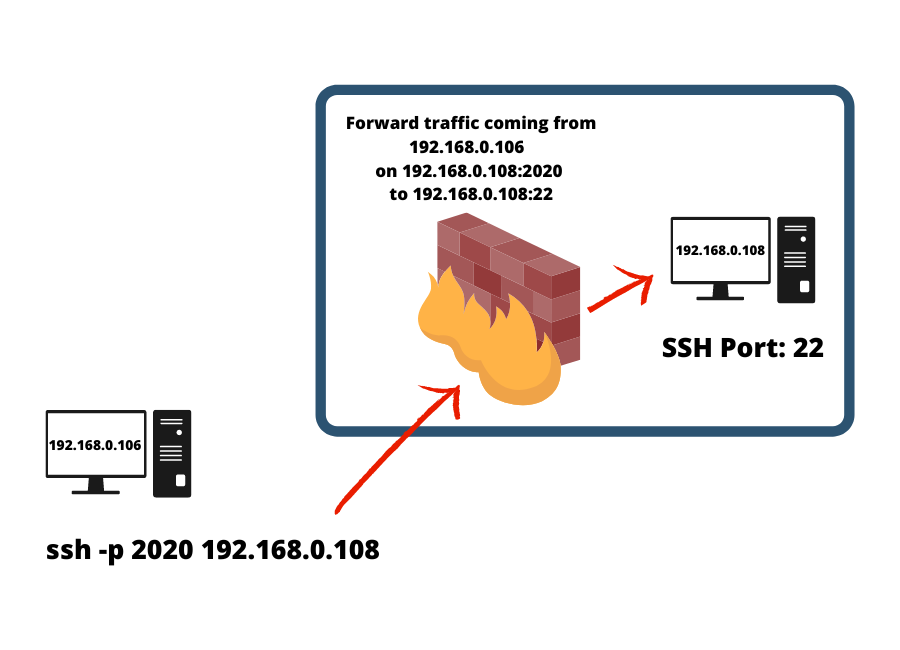
\includegraphics[scale=.52]{content/chapter2/images/port.png}
		\caption{Port forwarding}
		\label{fig:command_prompt12}
	\end{figure}
	
	\begin{tcolorbox}[breakable,notitle,boxrule=-0pt,colback=black,colframe=black]
			\color{green}
			\fontdimen2\font=1em
			\# firewall-cmd --permanent --add-rich-rule 'rule family=ipv4 source address=192.168.0.106/24 forward-port port=2020 protocol=tcp to-port=22'
			\newline
			\newline
			\# firewall-cmd --reload
			\fontdimen2\font=4pt
	\end{tcolorbox}
		
	
\end{itemize}

	
\end{flushleft}

\newpage





